% Options for packages loaded elsewhere
\PassOptionsToPackage{unicode}{hyperref}
\PassOptionsToPackage{hyphens}{url}
\PassOptionsToPackage{dvipsnames,svgnames,x11names}{xcolor}
%
\documentclass[
  a4paper,
]{scrreport}

\usepackage{amsmath,amssymb}
\usepackage{lmodern}
\usepackage{iftex}
\ifPDFTeX
  \usepackage[T1]{fontenc}
  \usepackage[utf8]{inputenc}
  \usepackage{textcomp} % provide euro and other symbols
\else % if luatex or xetex
  \usepackage{unicode-math}
  \defaultfontfeatures{Scale=MatchLowercase}
  \defaultfontfeatures[\rmfamily]{Ligatures=TeX,Scale=1}
\fi
% Use upquote if available, for straight quotes in verbatim environments
\IfFileExists{upquote.sty}{\usepackage{upquote}}{}
\IfFileExists{microtype.sty}{% use microtype if available
  \usepackage[]{microtype}
  \UseMicrotypeSet[protrusion]{basicmath} % disable protrusion for tt fonts
}{}
\makeatletter
\@ifundefined{KOMAClassName}{% if non-KOMA class
  \IfFileExists{parskip.sty}{%
    \usepackage{parskip}
  }{% else
    \setlength{\parindent}{0pt}
    \setlength{\parskip}{6pt plus 2pt minus 1pt}}
}{% if KOMA class
  \KOMAoptions{parskip=half}}
\makeatother
\usepackage{xcolor}
\setlength{\emergencystretch}{3em} % prevent overfull lines
\setcounter{secnumdepth}{5}
% Make \paragraph and \subparagraph free-standing
\ifx\paragraph\undefined\else
  \let\oldparagraph\paragraph
  \renewcommand{\paragraph}[1]{\oldparagraph{#1}\mbox{}}
\fi
\ifx\subparagraph\undefined\else
  \let\oldsubparagraph\subparagraph
  \renewcommand{\subparagraph}[1]{\oldsubparagraph{#1}\mbox{}}
\fi


\providecommand{\tightlist}{%
  \setlength{\itemsep}{0pt}\setlength{\parskip}{0pt}}\usepackage{longtable,booktabs,array}
\usepackage{calc} % for calculating minipage widths
% Correct order of tables after \paragraph or \subparagraph
\usepackage{etoolbox}
\makeatletter
\patchcmd\longtable{\par}{\if@noskipsec\mbox{}\fi\par}{}{}
\makeatother
% Allow footnotes in longtable head/foot
\IfFileExists{footnotehyper.sty}{\usepackage{footnotehyper}}{\usepackage{footnote}}
\makesavenoteenv{longtable}
\usepackage{graphicx}
\makeatletter
\def\maxwidth{\ifdim\Gin@nat@width>\linewidth\linewidth\else\Gin@nat@width\fi}
\def\maxheight{\ifdim\Gin@nat@height>\textheight\textheight\else\Gin@nat@height\fi}
\makeatother
% Scale images if necessary, so that they will not overflow the page
% margins by default, and it is still possible to overwrite the defaults
% using explicit options in \includegraphics[width, height, ...]{}
\setkeys{Gin}{width=\maxwidth,height=\maxheight,keepaspectratio}
% Set default figure placement to htbp
\makeatletter
\def\fps@figure{htbp}
\makeatother

\usepackage{pgfplots}
\usetikzlibrary{arrows.meta,arrows}
\usetikzlibrary{shapes.geometric}
\usetikzlibrary{angles,quotes}
\pgfplotsset{grid style={dashed,mygray}}
% Colors
\definecolor{myblue}{rgb}{0.067,0.529,0.871}
\definecolor{mypurple}{rgb}{0.859,0.071,0.525}
\definecolor{myred}{rgb}{1.0, 0.13, 0.32}
\definecolor{mygreen}{rgb}{0.01, 0.75, 0.24}
\definecolor{myblack}{gray}{0.1}
\definecolor{mygray}{gray}{0.8}
\newcommand{\NN}{\mathbb{N}}
\newcommand{\ZZ}{\mathbb{Z}}
\newcommand{\QQ}{\mathbb{Q}}
\newcommand{\RR}{\mathbb{R}}
\newcommand{\CC}{\mathbb{C}}
\DeclareMathOperator{\Int}{Int}
\DeclareMathOperator{\Ext}{Ext}
\DeclareMathOperator{\Fr}{Fr}
\DeclareMathOperator{\Adh}{Adh}
\DeclareMathOperator{\Ac}{Ac}
\DeclareMathOperator{\sen}{sen}
\makeatletter
\@ifpackageloaded{tcolorbox}{}{\usepackage[many]{tcolorbox}}
\@ifpackageloaded{fontawesome5}{}{\usepackage{fontawesome5}}
\definecolor{quarto-callout-color}{HTML}{909090}
\definecolor{quarto-callout-note-color}{HTML}{0758E5}
\definecolor{quarto-callout-important-color}{HTML}{CC1914}
\definecolor{quarto-callout-warning-color}{HTML}{EB9113}
\definecolor{quarto-callout-tip-color}{HTML}{00A047}
\definecolor{quarto-callout-caution-color}{HTML}{FC5300}
\definecolor{quarto-callout-color-frame}{HTML}{acacac}
\definecolor{quarto-callout-note-color-frame}{HTML}{4582ec}
\definecolor{quarto-callout-important-color-frame}{HTML}{d9534f}
\definecolor{quarto-callout-warning-color-frame}{HTML}{f0ad4e}
\definecolor{quarto-callout-tip-color-frame}{HTML}{02b875}
\definecolor{quarto-callout-caution-color-frame}{HTML}{fd7e14}
\makeatother
\makeatletter
\@ifpackageloaded{tikz}{}{\usepackage{tikz}}
\makeatother
\makeatletter
\@ifpackageloaded{bookmark}{}{\usepackage{bookmark}}
\makeatother
\makeatletter
\@ifpackageloaded{caption}{}{\usepackage{caption}}
\AtBeginDocument{%
\ifdefined\contentsname
  \renewcommand*\contentsname{Tabla de contenidos}
\else
  \newcommand\contentsname{Tabla de contenidos}
\fi
\ifdefined\listfigurename
  \renewcommand*\listfigurename{Listado de Figuras}
\else
  \newcommand\listfigurename{Listado de Figuras}
\fi
\ifdefined\listtablename
  \renewcommand*\listtablename{Listado de Tablas}
\else
  \newcommand\listtablename{Listado de Tablas}
\fi
\ifdefined\figurename
  \renewcommand*\figurename{Figura}
\else
  \newcommand\figurename{Figura}
\fi
\ifdefined\tablename
  \renewcommand*\tablename{Tabla}
\else
  \newcommand\tablename{Tabla}
\fi
}
\@ifpackageloaded{float}{}{\usepackage{float}}
\floatstyle{ruled}
\@ifundefined{c@chapter}{\newfloat{codelisting}{h}{lop}}{\newfloat{codelisting}{h}{lop}[chapter]}
\floatname{codelisting}{Listado}
\newcommand*\listoflistings{\listof{codelisting}{Listado de Listados}}
\usepackage{amsthm}
\theoremstyle{definition}
\newtheorem{exercise}{Ejercicio}[chapter]
\theoremstyle{remark}
\renewcommand*{\proofname}{Prueba}
\newtheorem*{remark}{Observación}
\newtheorem*{solution}{Solución}
\makeatother
\makeatletter
\@ifpackageloaded{caption}{}{\usepackage{caption}}
\@ifpackageloaded{subcaption}{}{\usepackage{subcaption}}
\makeatother
\makeatletter
\@ifpackageloaded{tcolorbox}{}{\usepackage[many]{tcolorbox}}
\makeatother
\makeatletter
\@ifundefined{shadecolor}{\definecolor{shadecolor}{rgb}{.97, .97, .97}}
\makeatother
\makeatletter
\makeatother
\ifLuaTeX
\usepackage[bidi=basic]{babel}
\else
\usepackage[bidi=default]{babel}
\fi
\babelprovide[main,import]{spanish}
% get rid of language-specific shorthands (see #6817):
\let\LanguageShortHands\languageshorthands
\def\languageshorthands#1{}
\ifLuaTeX
  \usepackage{selnolig}  % disable illegal ligatures
\fi
\IfFileExists{bookmark.sty}{\usepackage{bookmark}}{\usepackage{hyperref}}
\IfFileExists{xurl.sty}{\usepackage{xurl}}{} % add URL line breaks if available
\urlstyle{same} % disable monospaced font for URLs
\hypersetup{
  pdftitle={Exámenes de Análisis Matemático},
  pdfauthor={Alfredo Sánchez Alberca},
  pdflang={es},
  colorlinks=true,
  linkcolor={blue},
  filecolor={Maroon},
  citecolor={Blue},
  urlcolor={Blue},
  pdfcreator={LaTeX via pandoc}}

\title{Exámenes de Análisis Matemático}
\author{Alfredo Sánchez Alberca}
\date{11/1/22}

\begin{document}
\begin{titlepage}

%\AddToShipoutPicture*{\put(0,0){\includegraphics[scale=0.8]{img/background2}}} % Imagen de fondo, requiere el paquete eso-pic.
\begin{center}
\vspace*{5cm}

\Huge
{\textbf{\textsf{Exámenes de Análisis Matemático}}}

\vspace{0.5cm}
\LARGE
{\textbf{\textsf{}}}

\vspace{1.5cm}


\includegraphics[width=0.4\textwidth]{img/logos/sticker.png}
\end{center}

\vfill

\begin{flushleft}
\begin{tabular}{ll}

\includegraphics[width=0.1\textwidth]{img/logos/aprendeconalf.png} & \parbox[b]{5cm}{\Large\textsf{Alfredo
Sánchez
Alberca}\\ \textsf{asalber@ceu.es} \\ \textsf{https://aprendeconalf.es}}
\end{tabular}
\end{flushleft}
\end{titlepage}\ifdefined\Shaded\renewenvironment{Shaded}{\begin{tcolorbox}[interior hidden, boxrule=0pt, breakable, frame hidden, enhanced, borderline west={3pt}{0pt}{shadecolor}, sharp corners]}{\end{tcolorbox}}\fi

\renewcommand*\contentsname{Tabla de contenidos}
{
\hypersetup{linkcolor=}
\setcounter{tocdepth}{2}
\tableofcontents
}
\bookmarksetup{startatroot}

\hypertarget{prefacio}{%
\chapter*{Prefacio}\label{prefacio}}
\addcontentsline{toc}{chapter}{Prefacio}

\markboth{Prefacio}{Prefacio}

Colección de exámenes de Análisis Matemático Real del grado en
Ingeniería Matemática.

\bookmarksetup{startatroot}

\hypertarget{examen-de-anuxe1lisis-i-noviembre-2022}{%
\chapter{Examen de Análisis I (Noviembre
2022)}\label{examen-de-anuxe1lisis-i-noviembre-2022}}

\leavevmode\vadjust pre{\hypertarget{exr-1}{}}%
\begin{exercise}[]\label{exr-1}

Calcular los puntos de acumulación del conjunto
\(A=[0,1]\cup \left\{\frac{n}{n-1}: n\in\mathbb{N}, n\geq 2\right\}\).
¿Es un conjunto cerrado? ¿Y abierto?

\end{exercise}

\begin{tcolorbox}[enhanced jigsaw, toprule=.15mm, arc=.35mm, titlerule=0mm, opacityback=0, rightrule=.15mm, colbacktitle=quarto-callout-tip-color!10!white, bottomtitle=1mm, breakable, colback=white, opacitybacktitle=0.6, coltitle=black, left=2mm, toptitle=1mm, title=\textcolor{quarto-callout-tip-color}{\faLightbulb}\hspace{0.5em}{Tip}, bottomrule=.15mm, colframe=quarto-callout-tip-color-frame, leftrule=.75mm]

Veamos primero que todos los puntos del intervalo \([0,1]\) son puntos
de acumulación. Sea \(x\in[0,1]\). Entonces para cualquier
\(\varepsilon>0\), por la densidad de los números reales, el entorno
reducido \((x-\varepsilon,x+\varepsilon)\setminus\{x\}\) contiene puntos
de \([0,1]\), y por tanto \(x\) es un punto de acumulación de \([0,1]\).

Veamos ahora que el conjunto
\(B=\left\{\frac{n}{n-1}: n\in\mathbb{N}, n\geq 2\right\} = \left\{1+\frac{1}{n-1}: n\in\mathbb{N}, n\geq 2\right\}\)
solo tiene \(1\) como punto de acumulación. En primer lugar, \(1\) es
punto de acumulación, ya que para cualquier \(\varepsilon>0\),
\((1-\varepsilon, 1+\varepsilon)\setminus \{1\}\) contiene puntos de
\(A\). Para verlo, basta aplicar la propiedad arquimediana, por la que
existe \(n\in\mathbb{N}\) tal que \(\frac{1}{n}<\varepsilon\), de manera
que \(1+\frac{1}{n}<1+\varepsilon\), y por tanto
\((1-\varepsilon, 1+\varepsilon)\setminus \{1\}\cap B\neq \emptyset\).

Si \(x<1\), tomando \(\varepsilon=|x-1|\) el entorno reducido
\((x-\varepsilon, x+\varepsilon)\setminus\{x\}\) no contiene puntos de
\(B\). Del mismo modo, si \(x>2\), tomando \(\varepsilon=|x-2|\) el
entorno reducido \((x-\varepsilon, x+\varepsilon)\setminus\{x\}\)
tampoco contiene puntos de \(B\). Finalmente, si \(1<x\leq 2\), por la
propiedad arquimediana, existe \(n\in\mathbb{N}\) tal que
\(\frac{1}{n}\leq x<\frac{1}{n-1}\). Tomando
\(\varepsilon=\min(\{|x-\frac{1}{n}|,|x-\frac{1}{n-1}|\})\) también se
tiene que el entorno reducido
\((x-\varepsilon, x+\varepsilon)\setminus\{x\}\) no contiene puntos de
\(B\). Por tanto, \(1\) es el único punto de acumulación de \(B\).

Así pues, \(\operatorname{Ac}(A)=[0,1]\), y como
\(\operatorname{Ac}(A)\subseteq A\), \(A\) es cerrado ya que contienen a
todos sus puntos de acumulación (ver
\href{https://aprendeconalf.es/analisis-manual/topologia-reales.html\#thm-conjunto-cerrado-puntos-acumulacion}{teorema}),
y por tanto, no puede ser abierto ya que los únicos conjuntos cerrados y
abiertos a la vez son \(\mathbb{R}\) y \(\emptyset\).

\end{tcolorbox}

\leavevmode\vadjust pre{\hypertarget{exr-2}{}}%
\begin{exercise}[]\label{exr-2}

Dada la sucesión \(\left(\frac{1}{2^n}\right)_{n=1}^\infty\),

\begin{enumerate}
\def\labelenumi{\alph{enumi}.}
\tightlist
\item
  Calcular, si existen, el supremo, ínfimo, máximo y mínimo del conjunto
  de sus términos.
\item
  Demostrar que la sucesión converge a \(0\).
\end{enumerate}

\end{exercise}

\begin{tcolorbox}[enhanced jigsaw, toprule=.15mm, arc=.35mm, titlerule=0mm, opacityback=0, rightrule=.15mm, colbacktitle=quarto-callout-tip-color!10!white, bottomtitle=1mm, breakable, colback=white, opacitybacktitle=0.6, coltitle=black, left=2mm, toptitle=1mm, title=\textcolor{quarto-callout-tip-color}{\faLightbulb}\hspace{0.5em}{Solución}, bottomrule=.15mm, colframe=quarto-callout-tip-color-frame, leftrule=.75mm]

\begin{enumerate}
\def\labelenumi{\alph{enumi}.}
\item
  La sucesión es monótona decreciente, ya que \(\forall n\in\mathbb{N}\)
  \(2^n<2^{n+1}\), y por tanto,
  \(x_n=\frac{1}{2^n}<\frac{1}{2^{n+1}}=x_{n+1}\). Así pues, el primer
  término de la sucesión \(x_1=1/2\) es su máximo, y por tanto el
  supremo.

  Veamos ahora que \(0\) es ínfimo por reducción al absurdo. En primer
  lugar, \(0\) es una cota inferior de la sucesión, pues todos sus
  términos son positivos. Supongamos ahora que existe otra cota inferior
  \(c\in\mathbb{R}\) tal que \(c>0\). Por la propiedad arquimediana,
  existe \(n\in\mathbb{N}\) tal que \(\frac{1}{n}< c\). Ahora bien, como
  \(n<2^n\) \(\forall n\in\mathbb{N}\), se tiene que
  \(\frac{1}{2^n}<\frac{1}{n}< c\), por lo que el termino \(n\) de la
  sucesión es menor que \(c\), lo que contradice que sea cota inferior.
  Así pues, \(0\) es el ínfimo. Sin embargo, la sucesión no tiene
  mínimo, pues \(x_n\neq 0\) \(\forall n\in\mathbb{N}\).
\item
  Como la sucesión es monótona decreciente y está acotada inferiormente,
  por el
  \href{https://aprendeconalf.es/analisis-manual/sucesiones.html\#thm-convergencia-monotona}{teorema
  de la convergencia de una sucesión monónota} la sucesión converge y
  \(\lim_{n\to\infty}x_n = \inf(\{x_n:n\in\mathbb{N}\})=0\).
\end{enumerate}

\end{tcolorbox}

\leavevmode\vadjust pre{\hypertarget{exr-3}{}}%
\begin{exercise}[]\label{exr-3}

La rentabilidad de un bono cada año, en porcentaje, viene dada por la
sucesión recurrente \(x_1=3\) y \(x_{n+1}=\sqrt{\frac{x_n}{2}+3}\).
¿Hacia dónde converge la rentabilidad del bono a medida que pasa el
tiempo?

\end{exercise}

\begin{tcolorbox}[enhanced jigsaw, toprule=.15mm, arc=.35mm, titlerule=0mm, opacityback=0, rightrule=.15mm, colbacktitle=quarto-callout-tip-color!10!white, bottomtitle=1mm, breakable, colback=white, opacitybacktitle=0.6, coltitle=black, left=2mm, toptitle=1mm, title=\textcolor{quarto-callout-tip-color}{\faLightbulb}\hspace{0.5em}{Solución}, bottomrule=.15mm, colframe=quarto-callout-tip-color-frame, leftrule=.75mm]

Veamos que primero que la sucesión es monótona decreciente.
\(x_1=3>x_n= \sqrt{\frac{3}{2}+3} = 2.12\). Supongamos ahora que
\(x_{n-1}>x_n\). Entonces

\begin{align*}
x_{n-1}>x_n &\Rightarrow \frac{x_{n-1}} {2}>\frac{x_n}{2} \Rightarrow \frac{x_{n-1}}{2}+3>\frac{x_n}{2}+3\\  & \Rightarrow \sqrt{\frac{x_{n-1}}{2}+3}>\sqrt{\frac{x_n}{2}+3} \Rightarrow x_n>x_{n+1}.
\end{align*} \[
\]

Por otro lado, es fácil ver que la sucesión está acotada inferiormente
por \(0\) pues todos los términos son positivos. Así pues, por el
\href{https://aprendeconalf.es/analisis-manual/sucesiones.html\#thm-convergencia-monotona}{teorema
de la convergencia de una sucesión monónota}, la sucesión converge a un
número \(x\in\mathbb{R}\). Para calcular el límite, aprovechando la
recurrencia de la sucesión se tiene

\[
x=\lim_{n\to\infty} x_n = \lim_{n\to\infty} x_{n+1} = \lim_{n\to\infty} \sqrt{\frac{x_n}{2}+3} = \sqrt{\lim_{n\to\infty}\frac{x_n}{2}+3} = \sqrt{\frac{x}{2}+3}
\]

Así pues, se cumple que \(x=\sqrt{\frac{x}{2}+3}\), y de ello se deduce

\[
x=\sqrt{\frac{x}{2}+3} \Rightarrow x^2=\frac{x}{2}+3 \Rightarrow x^2-3 = \frac{x}{2} \Rightarrow 2x^2-x-6 =0,\]

y resolviendo la ecuación se tiene \(x=-3/2\) y \(x=2\). Como todos los
términos de la sucesión son positivos, es imposible que converja a
\(-3/2\), y por tanto la rentabilidad del bono converge al \(2\)\%.

\end{tcolorbox}

\leavevmode\vadjust pre{\hypertarget{exr-4}{}}%
\begin{exercise}[]\label{exr-4}

Demostrar, usando la definición de límite, que
\(\lim_{x\to 1}\frac{3x+1}{2}=2\).

\end{exercise}

\begin{tcolorbox}[enhanced jigsaw, toprule=.15mm, arc=.35mm, titlerule=0mm, opacityback=0, rightrule=.15mm, colbacktitle=quarto-callout-tip-color!10!white, bottomtitle=1mm, breakable, colback=white, opacitybacktitle=0.6, coltitle=black, left=2mm, toptitle=1mm, title=\textcolor{quarto-callout-tip-color}{\faLightbulb}\hspace{0.5em}{Solución}, bottomrule=.15mm, colframe=quarto-callout-tip-color-frame, leftrule=.75mm]

Para cualquier \(\varepsilon>0\) existe
\(\delta=\frac{2}{3}\varepsilon\), tal que si
\(|x-1|<\delta=\frac{2}{3}\varepsilon\) se tiene

\[
\left|\frac{3x+1}{2}-2\right|= \left|\frac{3x+1-4}{2}\right| = \left|\frac{3x-3}{2}\right| = \left|\frac{3(x-1)}{2}\right| = \frac{3}{2}|x-1|< \frac{3}{2}\frac{2}{3}\varepsilon = \varepsilon.
\]

\end{tcolorbox}

\leavevmode\vadjust pre{\hypertarget{exr-5}{}}%
\begin{exercise}[]\label{exr-5}

Sabiendo que \(\lim_{x\to 0}(1+x)^{1/x}=e\), demostrar que las
siguientes funciones son infinitésimos equivalentes en \(x=0\):

\begin{enumerate}
\def\labelenumi{\alph{enumi}.}
\tightlist
\item
  \(\ln(1+x)\) y \(x\).
\item
  \(e^x-1\) y \(x\).
\end{enumerate}

\end{exercise}

\begin{tcolorbox}[enhanced jigsaw, toprule=.15mm, arc=.35mm, titlerule=0mm, opacityback=0, rightrule=.15mm, colbacktitle=quarto-callout-tip-color!10!white, bottomtitle=1mm, breakable, colback=white, opacitybacktitle=0.6, coltitle=black, left=2mm, toptitle=1mm, title=\textcolor{quarto-callout-tip-color}{\faLightbulb}\hspace{0.5em}{Solución}, bottomrule=.15mm, colframe=quarto-callout-tip-color-frame, leftrule=.75mm]

Para que dos funciones \(f\) y \(g\) sean infinitésimos equivalentes en
\(x=0\) se tiene que cumplir que \(\lim_{x\to 0}\frac{f(x)}{g(x)}=1\).

\begin{enumerate}
\def\labelenumi{\alph{enumi}.}
\item
  \begin{align*}
  \lim_{x\to 0}\frac{\ln(1+x)}{x} &= \lim_{x\to 0}\frac{1}{x}\ln(1+x) = \lim_{x\to 0}\ln\left((1+x)^{1/x}\right)\\  
  &= \ln\left(\lim_{x\to 0} (1+x)^{1/x}\right) = \ln(e) = 1.
  \end{align*}
\item
  Haciendo uso del resultado anterior se tiene
\end{enumerate}

\[\lim_{x\to 0}\frac{e^x-1}{x} = \lim_{x\to 0}\frac{e^{\ln(x+1)}-1}{x} = \lim_{x\to 0}\frac{x+1-1}{x} = \lim_{x\to 0} \frac{x}{x} = \lim_{x\to 0} 1 = 1.\]

\end{tcolorbox}

\leavevmode\vadjust pre{\hypertarget{exr-6}{}}%
\begin{exercise}[]\label{exr-6}

Determinar las asíntotas de la función
\(f(x)=\ln\left(\frac{1}{x}+1\right)x^2\).

\end{exercise}

\begin{tcolorbox}[enhanced jigsaw, toprule=.15mm, arc=.35mm, titlerule=0mm, opacityback=0, rightrule=.15mm, colbacktitle=quarto-callout-tip-color!10!white, bottomtitle=1mm, breakable, colback=white, opacitybacktitle=0.6, coltitle=black, left=2mm, toptitle=1mm, title=\textcolor{quarto-callout-tip-color}{\faLightbulb}\hspace{0.5em}{Solución}, bottomrule=.15mm, colframe=quarto-callout-tip-color-frame, leftrule=.75mm]

El dominio de la función es
\(\operatorname{Dom}(f) = \mathbb{R}-[-1,0]\) de modo que solo puede
haber asíntotas verticales a la izquierda de \(-1\) o a la derecha de
\(0\). Veamos primero, qué pasa con el límite por la izquierda en
\(-1\).

\[
\lim_{x\to -1^-}f(x) = \lim_{x\to -1^-}\ln\left(\frac{1}{x}+1\right)x^2 = \ln\left(\frac{1}{-1}+1\right)(-1)^2 = \ln(0) = -\infty.
\]

Por tanto, \(f\) tiene una asíntota vertical por la izquierda en
\(x=-1\).

Veamos ahora, qué pasa con el límite por la derecha en \(0\).

\begin{align*}
\lim_{x\to 0^+}f(x) &= \lim_{x\to 0^+}\ln\left(\frac{1}{x}+1\right)x^2 = \lim_{x\to 0^+}\ln\left(\frac{x+1}{x}\right)x^2 \\ 
&= \lim_{x\to 0^+} (\ln(x+1)-\ln(x))x^2 \\ 
&= \lim_{x\to 0^+}\ln(x+1)x^2 - \lim_{x\to 0^+}\ln(x)x^2\\ 
&= \ln(0+1)0^2 - \lim_{x\to 0^+}\frac{\ln(x)}{1/x^2} \\
&= 0 - \lim_{x\to 0^+}\frac{(\ln(x))'}{(1/x^2)'} = -\lim_{x\to 0^+} \frac{1/x}{-2/x^3} = \tag{L'Hôpital}\\
&= -\lim_{x\to 0^+} \frac{x^3}{-2x} = \lim_{x\to 0^+}\frac{x^2}{2} = 0.
\end{align*}

Por lo tanto, \(f\) no tiene asíntota vertical en \(x=0\).

Para ver si hay asíntotas horizontales estudiamos los límites en el
infinito.

\begin{align*}
\lim_{x\to \infty} f(x) &= \lim_{x\to \infty}\ln\left(\frac{1}{x}+1\right)x^2 = \lim_{x\to\infty} \frac{\ln(x^{-1}+1)}{x^{-2}}\\ 
&= \lim_{x\to\infty} \frac{(\ln(x^{-1}+1))'}{(x^{-2})'} \tag{L'Hôpital} = \lim_{x\to\infty} \frac{\frac{1}{x^{-1}+1}(-1)x^{-2}}{-2x^{-3}}\\  
&= \lim_{x\to \infty} \frac{x}{2(x^{-1}+1)} = \infty.
\end{align*}

Por tanto, \(f\) no tiene asíntota horizontal en \(\infty\). Veamos
ahora qué ocurre en \(-\infty\).

\begin{align*}
\lim_{x\to -\infty} f(x) &= \lim_{x\to -\infty}\ln\left(\frac{1}{x}+1\right)x^2 = \lim_{x\to -\infty} \frac{\ln(x^{-1}+1)}{x^{-2}}\\ 
&= \lim_{x\to -\infty} \frac{(\ln(x^{-1}+1))'}{(x^{-2})'} \tag{L'Hôpital} = \lim_{x\to -\infty} \frac{\frac{1}{x^{-1}+1}(-1)x^{-2}}{-2x^{-3}}\\ 
&= \lim_{x\to -\infty} \frac{x}{2(x^{-1}+1)} = -\infty.
\end{align*}

Luego, \(f\) tampoco tiene asíntota vertical en \(-\infty\).

Finalmente, veamos si \(f\) tiene asíntotas oblicuas.

\begin{align*}
\lim_{x\to \infty} \frac{f(x)}{x} &= \lim_{x\to \infty}\frac{\ln\left(\frac{1}{x}+1\right)x^2}{x} = \lim_{x\to \infty}\ln\left(\frac{1}{x}+1\right)x \\
&= \lim_{x\to \infty} \ln\left(\left(\frac{1}{x}+1\right)^x\right) = \ln\left(\lim_{x\to \infty} \left(\frac{1}{x}+1\right)^x\right)\\ 
&= \ln(e)=1
\end{align*}

Por tanto, \(f\) tiene asíntota vertical en \(\infty\) con pendiente
\(b=1\). Para obtener el término independiente de la asíntota,
calculamos el siguiente límite.

\begin{align*}
\lim_{x\to \infty} f(x)-x &= \lim_{x\to \infty}\ln\left(\frac{1}{x}+1\right)x^2-x\\  
&= \lim_{x\to \infty}(\ln(x^{-1}+1)x-1)x \\
&= \lim_{x\to \infty}\frac{\ln(x^{-1}+1)x-1}{x^{-1}}\\  
&=  \lim_{x\to \infty}\frac{(\ln(x^{-1}+1)x-1)'}{(x^{-1})'} \tag{L'Hôpital} \\
&= \lim_{x\to \infty}\frac{\frac{-1}{(x^{-1}+1)x^2}x+\ln(x^{-1}+1)}{(-1)x^{-2}}\\ 
&= \lim_{x\to \infty}\frac{\frac{-1}{(x+1)}+\ln(x^{-1}+1)}{-x^{-2}} \\
&= \lim_{x\to \infty}\frac{\left(\frac{-1}{(1+x)}+\ln(x^{-1}+1)\right)'}{(-x^{-2})'}\\ 
&= \lim_{x\to \infty}\frac{\frac{1}{(x+1)^2}-\frac{1}{(x^{-1}+1)x^2}}{2x^{-3}}\tag{L'Hôpital}\\ 
&= \lim_{x\to \infty}\frac{\frac{1}{(x+1)^2}-\frac{1}{(x+1)x}}{2x^{-3}} = \lim_{x\to \infty}\frac{\frac{-1}{(x+1)^2x}}{2x^{-3}} \\
&= \lim_{x\to \infty}\frac{-x^3}{2(x^3+2x^2+x)} = \frac{-1}{2}
\end{align*}

Así pues, \(f\) tiene una asíntota oblicua \(y=x-\frac{1}{2}\) en
\(\infty\).

Del mismo modo se prueba que esta misma recta también es asíntota
oblicua de \(f\) en \(-\infty\).

\end{tcolorbox}

\bookmarksetup{startatroot}

\hypertarget{examen-de-anuxe1lisis-i-diciembre-2022}{%
\chapter{Examen de Análisis I (Diciembre
2022)}\label{examen-de-anuxe1lisis-i-diciembre-2022}}

\hypertarget{primera-parte}{%
\section{Primera parte}\label{primera-parte}}

\leavevmode\vadjust pre{\hypertarget{exr-1}{}}%
\begin{exercise}[]\label{exr-1}

La población de parásitos que infecta un árbol, en miles, evoluciona
diariamente siguiendo la sucesión recursiva \(x_1=2\) y
\(x_{n+1}=1-(2+x_n)^{-1}\) \(\forall n\in\mathbb{N}\). Demostrar que la
sucesión converge y calcular su límite.

\end{exercise}

\begin{tcolorbox}[enhanced jigsaw, toprule=.15mm, arc=.35mm, titlerule=0mm, opacityback=0, rightrule=.15mm, colbacktitle=quarto-callout-tip-color!10!white, bottomtitle=1mm, breakable, colback=white, opacitybacktitle=0.6, coltitle=black, left=2mm, toptitle=1mm, title=\textcolor{quarto-callout-tip-color}{\faLightbulb}\hspace{0.5em}{Solución}, bottomrule=.15mm, colframe=quarto-callout-tip-color-frame, leftrule=.75mm]

El término recurrente de la sucesión puede escribirse de la siguiente
manera

\[
x_{n+1}=1-(2+x_n)^{-1} = \frac{1+x_n}{2+x_n}\ \forall n\in\mathbb{N}.
\]

Veamos primero que la sucesión está acotada inferiormente por \(0\) por
inducción. \(x_1=2>0\), y suponiendo \(x_n>0\) se tiene que
\(x_{n+1} = \frac{1+x_n}{2+x_n} >0\) \(\forall n\in\mathbb{N}\).

Veamos ahora que la sucesión es decreciente también por inducción.
\(x_1 = 2 < x_2 = 1-(2+2)^{-1} = 3/4\). Supongamos ahora que
\(x_{n-1}>x_n\), entonces

\[
\begin{gathered}
x_{n-1}>x_n \Leftrightarrow 2+x_{n-1} > 2+x_n \Leftrightarrow (2+x_{n-1})^{-1} < (2+x_n)^{-1} \\
\Leftrightarrow 1-(2+x_{n-1})^{-1} > 1-(2+x_n)^{-1} \Leftrightarrow x_{n}>x_{n+1}\ \forall n\in\mathbb{N}.
\end{gathered}
\]

Así pues, como la sucesión es monótona decreciente y está acotada
inferiormente, según el
\href{https://aprendeconalf.es/analisis-manual/sucesiones.html\#thm-convergencia-monotona}{teorema
de la convergencia monótona}, la sucesión converge.

Para calcular el límite aprovechamos la recurrencia,

\[
x = \lim_{n\to\infty}x_n = \lim_{n\to\infty} \frac{1+x_{n-1}}{2+x_{n-1}} =\frac{1+\lim_{n\to\infty}x_{n-1}}{2+\lim_{n\to\infty}x_{n-1}} = \frac{1+x}{2+x},
\]

y resolviendo la ecuación se tiene

\[
x = \frac{1+x}{2+x} \Leftrightarrow x(2+x) = 1+x \Leftrightarrow x^2+x-1=0 \Leftrightarrow x = \frac{-1\pm \sqrt{5}}{2}.
\]

Como hemos visto que la sucesión está acotada inferiormente por \(0\),
podemos descartar la solución negativa, de manera que,
\(\lim_{n\to\infty}x_n = \frac{-1+ \sqrt{5}}{2}\).

\end{tcolorbox}

\leavevmode\vadjust pre{\hypertarget{exr-2}{}}%
\begin{exercise}[]\label{exr-2}

En el siglo III A.C usó el método por agotamiento para calcular el área
encerrada por una circunferencia. La idea consiste en inscribir la
circunferencia en polígonos regulares con un número de lados cada vez
mayor.

El área de estos polígonos puede calcularse fácilmente descomponiendo
los polígonos regulares en triángulos como en el siguiente ejemplo.

\begin{figure}

{\centering 

\usetikzlibrary{shapes.geometric}
\usetikzlibrary{angles}
\definecolor{myblue}{rgb}{0.067,0.529,0.871}
\definecolor{mypurple}{rgb}{0.859,0.071,0.525}
\definecolor{myred}{rgb}{1.0, 0.13, 0.32}
\definecolor{mygreen}{rgb}{0.01, 0.75, 0.24}
\def\PolyRadius{2cm}
\begin{tikzpicture}[draw=myblue, text=myblue]
\draw (0,0) circle (2);
\coordinate (A) at (-1,-1.74);
\coordinate (B) at (0,0);
\coordinate (C) at (1,-1.74);
\fill[fill=red!20] (0,0) -- (-1,-1.74) -- (1, -1.74) -- (0,0);
\node[regular polygon,draw,regular polygon sides = 6,minimum size=2*\PolyRadius] at (0,0) {};
\draw pic[draw,angle radius=0.5cm]{angle=A--B--C};
\node at (0,-0.35) {\scriptsize $\alpha$};
\draw [dashed] (0,0) -- (2,0);
\draw [dashed] (0,0) -- (-2,0);
\draw [dashed] (0,0) -- (1,1.74);
\draw [dashed] (0,0) -- (-1,1.74);
\draw [dashed] (0,0) -- (-1,-1.74);
\draw [dashed] (0,0) -- (1,-1.74) node[right, midway] {$r$};
\end{tikzpicture}


}

\caption{Descomposición de un hexágono en triángulos}

\end{figure}

\begin{enumerate}
\def\labelenumi{\alph{enumi}.}
\item
  Dar el término general de la sucesión \((a_n)_{n=3}^\infty\) que
  expresa el área del polígono en función del número de lados \(n\).
\item
  Calcular el límite de la sucesión.
\end{enumerate}

\end{exercise}

\begin{tcolorbox}[enhanced jigsaw, toprule=.15mm, arc=.35mm, titlerule=0mm, opacityback=0, rightrule=.15mm, colbacktitle=quarto-callout-tip-color!10!white, bottomtitle=1mm, breakable, colback=white, opacitybacktitle=0.6, coltitle=black, left=2mm, toptitle=1mm, title=\textcolor{quarto-callout-tip-color}{\faLightbulb}\hspace{0.5em}{Solución}, bottomrule=.15mm, colframe=quarto-callout-tip-color-frame, leftrule=.75mm]

\begin{enumerate}
\def\labelenumi{\alph{enumi}.}
\tightlist
\item
  Consideremos cada uno de los triángulos en los que se puede
  descomponer un polígono regular de \(n\) lados.
\end{enumerate}

\begin{figure}[H]

{\centering 

\usetikzlibrary{shapes.geometric}
\usetikzlibrary{angles}
\definecolor{myblue}{rgb}{0.067,0.529,0.871}
\definecolor{mypurple}{rgb}{0.859,0.071,0.525}
\definecolor{myred}{rgb}{1.0, 0.13, 0.32}
\definecolor{mygreen}{rgb}{0.01, 0.75, 0.24}
\begin{tikzpicture}[draw=myblue, text=myblue]
\coordinate (A) at (-1,-1.74);
\coordinate (B) at (0,0);
\coordinate (C) at (1,-1.74);
\draw pic[draw, angle radius=0.5cm]{angle=A--B--C};
\node at (0,-0.25) {$\alpha$};
\draw (C) -- (A) -- (B) -- (C) node[right, midway] {$r$};
\draw (B) -- (0,-1.74) node[left, midway] {$a$};
\draw (0, -1.74) -- (C) node[below, midway] {$b$}; 
\end{tikzpicture}


}

\caption{Dimensiones del triángulo}

\end{figure}

Puesto que para un polígono de \(n\) lados se obtienen \(n\) triángulos
iguales, se tiene que el ángulo \(\alpha=\frac{2\pi}{n}\) de manera que
\(\frac{\alpha}{2} = \frac{\pi}{n}\).

Aplicando las razones trigonométricas de un triángulo rectángulo, se
puede deducir que

\begin{align*}
\cos(\alpha/2) &= \cos(\pi/n) = \frac{a}{r} \Rightarrow a = r\cos(\pi/n)\\
\operatorname{sen}(\alpha/2) &= \operatorname{sen}(\pi/n) = \frac{b}{r} \Rightarrow b = r\operatorname{sen}(\pi/n)
\end{align*}

Por tanto, el área del triángulo es

\[
\frac{a2b}{2} = ab= r^2\cos(\pi/n)\operatorname{sen}(\pi/n),
\]

y como hay \(n\) triángulos idénticos en el polígono regular de \(n\)
lados, se tiene que el área del polígono es

\[
a_n  = n r^2\cos(\pi/n)\operatorname{sen}(\pi/n)
\]

\begin{enumerate}
\def\labelenumi{\alph{enumi}.}
\setcounter{enumi}{1}
\item
  Calculamos ahora el límite de la sucesión

  \begin{align*}
   \lim_{n\to\infty} a_n &= \lim_{n\to\infty} n r^2\cos(\pi/n)\operatorname{sen}(\pi/n)\\ 
   &= r^2 \lim_{n\to\infty}\cos(\pi/n)\lim_{n\to\infty}n\operatorname{sen}(\pi/n) \\ 
   &= r^2 \cos(0)\lim_{n\to\infty}\pi\frac{n}{\pi}\operatorname{sen}(\pi/n) \\ 
   &= \pi r^2 \lim_{n\to\infty}\frac{\operatorname{sen}(\pi/n)}{\pi/n} \\
   &= \pi r^2 \lim_{\pi/n\to 0} \frac{\operatorname{sen}(\pi/n)}{\pi/n} = \pi r^2, \tag{$\operatorname{sen}(\pi/n)\approx \pi/n$}
   \end{align*}

  que efectivamente es el área del círculo de radio \(r\).
\end{enumerate}

\end{tcolorbox}

\leavevmode\vadjust pre{\hypertarget{exr-3}{}}%
\begin{exercise}[]\label{exr-3}

Sabiendo que \(\operatorname{sen}(x)\) y \(x\) son infinitésimos
equivalentes en \(x=0\), demostrar que también lo son
\(\operatorname{tg}(x)\) y \(x\).

\end{exercise}

\begin{tcolorbox}[enhanced jigsaw, toprule=.15mm, arc=.35mm, titlerule=0mm, opacityback=0, rightrule=.15mm, colbacktitle=quarto-callout-tip-color!10!white, bottomtitle=1mm, breakable, colback=white, opacitybacktitle=0.6, coltitle=black, left=2mm, toptitle=1mm, title=\textcolor{quarto-callout-tip-color}{\faLightbulb}\hspace{0.5em}{Solución}, bottomrule=.15mm, colframe=quarto-callout-tip-color-frame, leftrule=.75mm]

Como \(\operatorname{sen}(x)\) y \(x\) son infinitésimos equivalentes en
\(x=0\), se tiene que
\(\lim_{x\to 0}\frac{\operatorname{sen}(x)}{x} = 1\).

Para demostrar que \(\operatorname{tg}(x)\) y \(x\) también son
infinitésimos equivalentes en \(x=0\) calculamos el límite

\begin{align*}
\lim_{x\to 0}\frac{\operatorname{tg}(x)}{x} &= \lim_{x\to 0}\frac{\frac{\operatorname{sen}(x)}{\cos(x)}}{x} = \lim_{x\to 0}\frac{1}{\cos(x)}\frac{\operatorname{sen}(x)}{x} \\
&= \lim_{x\to 0}\frac{1}{\cos(x)}\lim_{x\to 0}\frac{\operatorname{sen}(x)}{x} = \lim_{x\to 0}\frac{1}{\cos(x)} 1 = \frac{1}{\cos(0)} = 1.
\end{align*}

Por tanto, \(\operatorname{tg}(x)\) y \(x\) son infinitésimos
equivalentes en \(x=0\).

\end{tcolorbox}

\leavevmode\vadjust pre{\hypertarget{exr-4}{}}%
\begin{exercise}[]\label{exr-4}

Determinar el dominio y el tipo de asíntotas de la función

\[f(x)=\sqrt{\frac{x^3}{4x-1}}.\]

\end{exercise}

\begin{tcolorbox}[enhanced jigsaw, toprule=.15mm, arc=.35mm, titlerule=0mm, opacityback=0, rightrule=.15mm, colbacktitle=quarto-callout-tip-color!10!white, bottomtitle=1mm, breakable, colback=white, opacitybacktitle=0.6, coltitle=black, left=2mm, toptitle=1mm, title=\textcolor{quarto-callout-tip-color}{\faLightbulb}\hspace{0.5em}{Solución}, bottomrule=.15mm, colframe=quarto-callout-tip-color-frame, leftrule=.75mm]

Para que exista la raíz, el radicando debe ser positivo, es decir,
\(\frac{x^3}{4x-1}\geq 0\). Es fácil ver que
\(x^3\geq 0\Leftrightarrow x\geq 0\) y
\(4x-1\geq 0\Leftrightarrow x\geq 1/4\) de manera que
\(\frac{x^3}{4x-1}\geq 0\Leftrightarrow x\leq 0 \mbox{ o } x\geq 1/4\).

Por otro lado, para que exista \(\frac{x^3}{4x-1}\) el denominador no
puede anularse, es decir \(4x-1\neq 0 \Leftrightarrow x\neq 1/4\). Por
tanto, concluimos que el dominio de la función es
\(\operatorname{Dom}(f)=(-\infty, 0]\cup (\frac{1}{4},\infty)\).

Estudiamos ahora los tipos de asíntotas que tiene la función.

\textbf{Asíntotas verticales}

Los únicos puntos donde pueden existir asíntotas verticales son \(x=0\)
y \(x=1/4\), así que calculamos los límites laterales en estos puntos.

\[
\lim_{x\to 0^-}f(x) = \lim_{x\to 0^-} \sqrt{\frac{x^3}{4x-1}} = \sqrt{\frac{0^3}{4\cdot 0-1}} = 0,
\]

y por tanto, \(f\) no tiene asíntota vertical en \(x=0\).

\[
\lim_{x\to 1/4^+}f(x) = \lim_{x\to 1/4^+} \sqrt{\frac{x^3}{4x-1}} = \sqrt{\frac{(1/4)^3}{4(1/4)-1}} = \infty,
\]

y por tanto, \(f\) tiene una asíntota vertical en \(x=1/4\).

\textbf{Asíntotas horizontales}

Para ver si hay asíntotas horizontales estudiamos los límites en
\(\pm \infty\).

\begin{align*}
\lim_{x\to-\infty}f(x) &=  \lim_{x\to-\infty} \sqrt{\frac{x^3}{4x-1}} = \lim_{x\to-\infty} \sqrt{\frac{\frac{x^3}{x}}{\frac{4x-1}{x}}} = \lim_{x\to-\infty} \sqrt{\frac{x^2}{4-\frac{1}{x}}} = \infty.\\
\lim_{x\to\infty}f(x) &=  \lim_{x\to\infty} \sqrt{\frac{x^3}{4x-1}} = \lim_{x\to\infty} \sqrt{\frac{\frac{x^3}{x}}{\frac{4x-1}{x}}} = \lim_{x\to\infty} \sqrt{\frac{x^2}{4-\frac{1}{x}}} = \infty.
\end{align*}

Por tanto, \(f\) no tiene asíntotas horizontales.

\textbf{Asíntotas oblicuas}

Para ver si hay asíntotas oblicuas estudiamos los límites de \(f(x)/x\)
en \(\pm\infty\)

\begin{align*}
\lim_{x\to-\infty}\frac{f(x)}{x} &=  \lim_{x\to-\infty} \frac{\sqrt{\frac{x^3}{4x-1}}}{x} = \lim_{x\to-\infty} \sqrt{\frac{x^3}{4x^3-x^2}} = \sqrt{\frac{1}{4}} = \frac{-1}{2}\\
\lim_{x\to\infty}\frac{f(x)}{x} &=  \lim_{x\to\infty} \frac{\sqrt{\frac{x^3}{4x-1}}}{x} = \lim_{x\to\infty} \sqrt{\frac{x^3}{4x^3-x^2}} = \sqrt{\frac{1}{4}} = \frac{1}{2}
\end{align*}

Por tanto, \(f\) tiene asíntotas oblicuas tanto en \(-\infty\) como en
\(\infty\).

\end{tcolorbox}

\leavevmode\vadjust pre{\hypertarget{exr-5}{}}%
\begin{exercise}[]\label{exr-5}

Dado el conjunto \(A=\{x\in\mathbb{R} : \frac{x^2-1}{x-2}\leq 0\}\),
calcular, si existe, el supremo, ínfimo, máximo y mínimo. ¿Es un
conjunto cerrado o abierto?

\end{exercise}

\begin{tcolorbox}[enhanced jigsaw, toprule=.15mm, arc=.35mm, titlerule=0mm, opacityback=0, rightrule=.15mm, colbacktitle=quarto-callout-tip-color!10!white, bottomtitle=1mm, breakable, colback=white, opacitybacktitle=0.6, coltitle=black, left=2mm, toptitle=1mm, title=\textcolor{quarto-callout-tip-color}{\faLightbulb}\hspace{0.5em}{Solución}, bottomrule=.15mm, colframe=quarto-callout-tip-color-frame, leftrule=.75mm]

\(A\) puede expresarse con la unión de intervalos, ya que
\(x^2-1\geq 0 \Leftrightarrow x^2\geq 1 \Leftrightarrow x\leq -1 \mbox{ o } x\geq 1\),
y por otro lado, \(x-2\geq 0 \Leftrightarrow x\geq 2\), de manera que
\(\frac{x^2-1}{x-2}\leq 0 \Leftrightarrow x\leq -1\) o \(1\leq x<2\), es
decir, \(A=(-\infty,-1]\cup [1,2)\).

Es fácil ver que \(A\) está acotado superiormente y la menor de las
cotas superiores es \(2\), por lo que el supremo es \(2\), pero como
\(2\not\in A\), \(A\) no tiene máximo.

En cuanto al ínfimo, \(A\) no está acotado inferiormente, de manera que
no tiene ínfimo, y por tanto, tampoco mínimo.

\(A\) no es abierto, ya que \(-1\in A\), pero \(-1\) no es un punto
interior de A, ya que para cualquier \(\varepsilon>0\) el intervalo
\((-1-\varepsilon,-1+\varepsilon)\) contiene puntos de \(\overline{A}\).

Por otro lado, \(A\) tampoco es cerrado ya que
\(\overline{A}=(-1,1)\cup [2,\infty)\) no es abierto, pues
\(2\in\overline{A}\) pero no es un punto interior suyo, ya que para
cualquier \(\varepsilon>0\) el intervalo
\((2-\varepsilon,2+\varepsilon)\) contiene puntos de \(A\).

\end{tcolorbox}

\hypertarget{segunda-parte}{%
\section{Segunda parte}\label{segunda-parte}}

\leavevmode\vadjust pre{\hypertarget{exr-6}{}}%
\begin{exercise}[]\label{exr-6}

Dar una aproximación de \(\ln(\sqrt{1/2})\) usando un polinomio de
Taylor de cuarto grado.

\end{exercise}

\begin{tcolorbox}[enhanced jigsaw, toprule=.15mm, arc=.35mm, titlerule=0mm, opacityback=0, rightrule=.15mm, colbacktitle=quarto-callout-tip-color!10!white, bottomtitle=1mm, breakable, colback=white, opacitybacktitle=0.6, coltitle=black, left=2mm, toptitle=1mm, title=\textcolor{quarto-callout-tip-color}{\faLightbulb}\hspace{0.5em}{Solución}, bottomrule=.15mm, colframe=quarto-callout-tip-color-frame, leftrule=.75mm]

Para realizar la aproximación que se pide calcularemos el polinomio de
Taylor de cuarto grado de la función \(f(x)=\ln(\sqrt{x})\) en el punto
\(1\), ya que el valor de la función y sus sucesivas derivadas en este
punto son sencillas. La fórmula del polinomio de Taylor es

\[
P_{f,1}^4(x) = f(1)+f'(1)(x-1)+\frac{f''(1)}{2!}(x-1)^2+\frac{f'''(1)}{3!}(x-1)^3+\frac{f''''(1)}{4!}(x-1)^4.
\]

Así pues, calculamos hasta la cuarta derivada en \(1\):

\[\renewcommand{\arraystretch}{1.5} 
\begin{array}{lll}
f(x)=\ln(\sqrt{x})=\frac{1}{2}\ln(x) & \quad & f(1) = \frac{1}{2}\ln(1) = 0\\
f'(x) = \frac{1}{2}x^{-1} & & f'(1) = \frac{1}{2}\\
f''(x) = \frac{-1}{2}x^{2} & & f''(1) = \frac{-1}{2}\\
f'''(x) = x^{-3} & & f'''(1) = 1\\
f''''(x) = -3x^{-4} & & f''''(1) = -3
\end{array}
\]

Y sustituyendo en la fórmula del polinomio de Taylor se tiene

\[
\begin{aligned} 
P_{f,1}^4(x) &= 0+\frac{1}{2}(x-1)+\frac{-1/2}{2}(x-1)^2+\frac{1}{6}(x-1)^3+\frac{-3}{24}(x-1)^4\\
&= \frac{1}{2}(x-1)-\frac{1}{4}(x-1)^2+\frac{1}{6}(x-1)^3-\frac{1}{8}(x-1)^4. \end{aligned}
\]

Para aproximar \(\ln(\sqrt{1/2})\) calculamos el polinomio en \(x=1/2\).

\[
P_{f,1}^4(1/2) = \frac{1}{2}\left(\frac{1}{2}-1\right)-\frac{1}{4}\left(\frac{1}{2}-1\right)^2+\frac{1}{6}\left(\frac{1}{2}-1\right)^3-\frac{1}{8}\left(\frac{1}{2}-1\right)^4 = -0.34114583.
\]

\end{tcolorbox}

\leavevmode\vadjust pre{\hypertarget{exr-7}{}}%
\begin{exercise}[]\label{exr-7}

La función \(h(x)=\dfrac{x^2-2x+a}{x^3+bx^2-6x}\) tiene una
discontinuidad evitable en \(x=2\). Calcular el valor de \(a\) y \(b\),
y clasificar el resto de discontinuidades.

\end{exercise}

\begin{tcolorbox}[enhanced jigsaw, toprule=.15mm, arc=.35mm, titlerule=0mm, opacityback=0, rightrule=.15mm, colbacktitle=quarto-callout-tip-color!10!white, bottomtitle=1mm, breakable, colback=white, opacitybacktitle=0.6, coltitle=black, left=2mm, toptitle=1mm, title=\textcolor{quarto-callout-tip-color}{\faLightbulb}\hspace{0.5em}{Solución}, bottomrule=.15mm, colframe=quarto-callout-tip-color-frame, leftrule=.75mm]

Para que la función \(h(x)=\dfrac{x^2-2x+a}{x^3+bx^2-6x}\) tenga una
discontinuidad evitable en \(x=2\), debe cumplirse que
\(\lim_{x\to 2}h(x)\neq h(2)\). Una manera de que esto se cumpla es que
la función no esté definida en \(x=2\) pero sí exista el límite en ese
punto. Para que la función no esté definida en \(x=2\) el denominador
debe anularse, es decir,

\[
2^3+b2^2-6\cdot 2=0\Rightarrow 8+4b-12 =0 \Rightarrow b=1.
\]

Por otro lado, el límite en \(x=2\) es

\[
\lim_{x\to 2}\frac{x^2-2x+a}{x^3+x^2-6x} = \frac{a}{0},
\]

de manera que, para que el límite exista, debe ser \(a=0\), y en tal
caso,

\[
\lim_{x\to 2}\frac{x^2-2x}{x^3+x^2-6x} = \lim_{x\to 2}\frac{x(x-2)}{x(x-2)(x+3)} = \lim_{x\to 2}\frac{1}{x+3} = \frac{1}{5},
\]

y, por tanto, \(h(x)\) tiene una discontinuidad evitable en \(x=2\) como
se pide.

Como se trata de una función racional, será discontinua en los puntos
que anulen el denominador, es decir \(x=-3\), \(x=0\) y \(x=2\). Ya
hemos visto que en \(x=2\) hay una discontinuidad evitable y faltaría
clasificar las otras dos discontinuidades.

En \(x=-3\) se tiene

\[
\begin{aligned} 
\lim_{x\to -3^-}\frac{x(x-2)}{x(x-2)(x+3)} &= \lim_{x\to -3^-}\frac{1}{x+3} = -\infty,\\
\lim_{x\to -3^+}\frac{x(x-2)}{x(x-2)(x+3)} &= \lim_{x\to -3^+}\frac{1}{x+3} = \infty, 
\end{aligned}
\]

y, por tanto, \(h\) tiene una discontinuidad de salto infinito en
\(x=-3\).

Finalmente en \(x=0\) se tiene

\[\lim_{x\to 0} \frac{x(x-2)}{x(x-2)(x+3)} = \lim_{x\to 0}\frac{1}{x+3} = \frac{1}{3},\]

por lo que \(h\) tiene otra discontinuidad evitable en \(x=0\).

\end{tcolorbox}

\leavevmode\vadjust pre{\hypertarget{exr-8}{}}%
\begin{exercise}[]\label{exr-8}

El envoltorio de unas píldoras está formado por un cilindro con dos
semiesferas en sus extremos, tal y como se aprecia en la imagen.

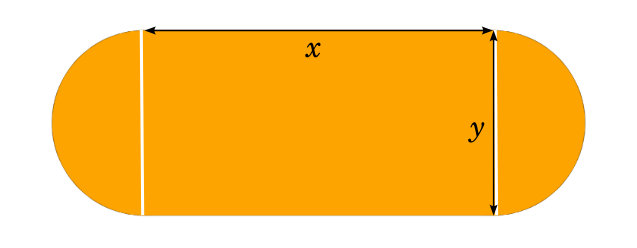
\includegraphics[width=8cm,height=3cm]{./img/examen-2022-12-21/pildora.png}

Si el contenido de las píldoras debe ser de \(0.15\) ml, hallar las
dimensiones de \(x\) e \(y\) para que el material empleado en el
envoltorio sea mínimo.

\end{exercise}

\begin{tcolorbox}[enhanced jigsaw, toprule=.15mm, arc=.35mm, titlerule=0mm, opacityback=0, rightrule=.15mm, colbacktitle=quarto-callout-tip-color!10!white, bottomtitle=1mm, breakable, colback=white, opacitybacktitle=0.6, coltitle=black, left=2mm, toptitle=1mm, title=\textcolor{quarto-callout-tip-color}{\faLightbulb}\hspace{0.5em}{Solución}, bottomrule=.15mm, colframe=quarto-callout-tip-color-frame, leftrule=.75mm]

El volumen de una esfera de radio \(r\) es \(v_e(r)=\frac{4}{3}\pi r^3\)
y el de un cilindro de radio \(r\) y altura \(h\) es
\(v_c(r,h)=\pi r^2 h\), de modo que que el volumen de la píldora es
\(v(r,h)=v_e(r)+v_c(r,h) = \frac{4}{3}\pi r^3 + \pi r^2 h\). Como el
volumen de la píldora debe ser \(0.15\) ml \(=0.15\) cm\(^3\),
imponiendo esta restricción, se tiene

\begin{equation}\protect\hypertarget{eq-cont-01-gen-eq1}{}{
v(r,h)=\frac{4}{3}\pi r^3 + \pi r^2 h = 0.15 \Leftrightarrow h = \frac{0.15-\frac{4}{3}\pi r^3}{\pi r^2}.
}\label{eq-cont-01-gen-eq1}\end{equation}

Por otro lado, la superficie de una esfera de radio \(r\) es
\(s_e(r)=4\pi r^2\) y la superficie del envolvente de un cilindro de
radio \(r\) y altura \(h\) es, en realidad, la superficie de un
rectángulo de lados \(2\pi r\) y \(h\), es decir,
\(s_c(r,h) = 2\pi r h\), de manera que la superficie de la píldora es
\(s(r,h) = 4\pi r^2+2\pi r h\), pero sustituyendo el valor de \(h\) que
hemos obtenido de imponer la restricción del volumen se tiene,

\begin{align*}
s(r) &= 4\pi r^2 + 2\pi r \left(\frac{0.15-\frac{4}{3}\pi r^3}{\pi r^2}\right) = 4\pi r^2 + \left(\frac{0.3-\frac{8}{3}\pi r^3}{r}\right)\\ 
&= 4\pi r^2 + \frac{0.3}{r} - \frac{8}{3}\pi r^2 = \frac{4}{3}\pi r^2+ \frac{0.3}{r},
\end{align*}

que es la función a optimizar.

Para calcular el mínimo de la función, calculamos primero los puntos
críticos.

\[
s'(r) = \frac{4}{3}\pi 2r -\frac{0.3}{r^2} =0 \Leftrightarrow \frac{8}{3}\pi r = \frac{0.3}{r^2} \Leftrightarrow r^3 = \frac{0.9}{8\pi} \Leftrightarrow r = \sqrt[3]{\frac{0.9}{8\pi}} \approx 0.3296 \mbox{cm}.
\]

Para ver si en este punto hay un mínimo aplicamos el
\href{https://aprendeconalf.es/analisis-manual/derivadas.html\#thm-concavidad}{criterio
de la segunda derivada}.

\[
s''(r) = \frac{8}{3}\pi -\frac{0.3(-2)}{r^3} =\frac{8}{3}\pi+\frac{0.6}{r^3} >0\ \forall r>0.
\]

Por tanto, \(s\) tiene un mínimo local en \(r=0.3296\), y la altura del
la píldora con la mínima superficie será, utilizando la
Ecuación~\ref{eq-cont-01-gen-eq1},

\[h =\frac{0.15-\frac{4}{3}\pi 0.3296^3}{\pi 0.3296^2}\approx 0.\]

Así pues, las dimensiones óptimas serían \(x=h=0\) cm e \(y=2r=0.6592\)
cm, que en realidad es una esfera de diámetro \(0.6592\) cm.

\end{tcolorbox}

\leavevmode\vadjust pre{\hypertarget{exr-9}{}}%
\begin{exercise}[]\label{exr-9}

Demostrar que la función
\(f(x)=\ln\left(k\left(x^2-2x+\frac{3}{2}\right)\right)\) no puede tener
más de una raíz en el intervalo \((0,1)\) para cualquier valor de \(k\).

\end{exercise}

\begin{tcolorbox}[enhanced jigsaw, toprule=.15mm, arc=.35mm, titlerule=0mm, opacityback=0, rightrule=.15mm, colbacktitle=quarto-callout-tip-color!10!white, bottomtitle=1mm, breakable, colback=white, opacitybacktitle=0.6, coltitle=black, left=2mm, toptitle=1mm, title=\textcolor{quarto-callout-tip-color}{\faLightbulb}\hspace{0.5em}{Solución}, bottomrule=.15mm, colframe=quarto-callout-tip-color-frame, leftrule=.75mm]

\(x^2-2x+\frac{3}{2}>0\) \(\forall x\in\mathbb{R}\), de manera que, para
que exista la función \(f\), debe ser también \(k>0\) y, por tanto,
aplicando propiedades de logaritmos se tiene,
\(f(x)=\ln\left(k\left(x^2-2x+\frac{3}{2}\right)\right)= \ln(k)+\ln\left(x^2-2x+\frac{3}{2}\right)\).

Por otro lado, como \(x^2-2x+\frac{3}{2}\) es un polinomio, es continuo
en todo \(\mathbb{R}\), y por tanto, \(f(x)\) también es continua en
todo \(\mathbb{R}\), siempre que \(k>0\).

Demostraremos que \(f\) no puede tener más de una raíz en el intervalo
\((0,1)\) por reducción al absurdo. Supongamos que existen
\(0 < a < b < 1\) tales que \(f(a)=f(b)=0\). Entonces, aplicando el
\href{https://aprendeconalf.es/analisis-manual/derivadas.html\#thm-rolle}{teorema
de Rolle}, debe existir algún valor \(c\in(a,b)\) tal que \(f'(c)=0\).
Si calculamos los puntos críticos de \(f\) se tiene

\[
f'(x) = \frac{2x-2}{x^2-2x+3/2} = 0 \Leftrightarrow 2x-2=0 \Leftrightarrow x=1,
\]

pero como \(1\not \in (a,b)\), llegamos a una contradicción ya que no
existe ningún valor \(c\in(a,b)\) con \(f'(c)=0\). Así pues, \(f\) no
puede tener más de una raíz en el intervalo \((0,1)\).

\end{tcolorbox}

\leavevmode\vadjust pre{\hypertarget{exr-10}{}}%
\begin{exercise}[]\label{exr-10}

Calcular las ecuaciones de las rectas tangente y normal a la gráfica de
la curva implícita \(e^{x^2y}-\ln(\sqrt{x-y})= 0\) en el punto \(x=0\).

\end{exercise}

\begin{tcolorbox}[enhanced jigsaw, toprule=.15mm, arc=.35mm, titlerule=0mm, opacityback=0, rightrule=.15mm, colbacktitle=quarto-callout-tip-color!10!white, bottomtitle=1mm, breakable, colback=white, opacitybacktitle=0.6, coltitle=black, left=2mm, toptitle=1mm, title=\textcolor{quarto-callout-tip-color}{\faLightbulb}\hspace{0.5em}{Solución}, bottomrule=.15mm, colframe=quarto-callout-tip-color-frame, leftrule=.75mm]

En primer lugar obtenemos los valores de \(y\) que cumplen la ecuación
de la curva implícita para \(x=0\). Sustituyendo en la ecuación se tiene

\[\begin{gathered} e^{0^2y}-\ln(\sqrt{0-y})= 0 \Leftrightarrow 1-\ln(\sqrt{-y}) = 0 \Leftrightarrow \\
\ln(\sqrt{-y}) = 1 \Leftrightarrow  \sqrt{-y} = e \Leftrightarrow y=-e^2. \end{gathered}\]

Así pues, hay que calcular la ecuación de las rectas tangente y normal
en el punto \((0,-e^2)\).

Como la pendiente de la recta tangente es la tasa de variación
instantánea, calculamos \(y'=\frac{dy}{dx}\) implícitamente

\[\begin{gathered} \left(e^{x^2y}-\ln(\sqrt{x-y})\right)'= 0' \Leftrightarrow \left(e^{x^2y}-\frac{1}{2}\ln(x-y)\right)'= 0 \Leftrightarrow \\
e^{x^2y}(2xy+x^2y')-\frac{1}{2}\frac{1-y'}{x-y} = 0. \end{gathered}\]

Sustituyendo en \(x=0\) y \(y=-e^2\), se tiene

\[\begin{gathered} e^{0^2(-e^2)}(2\cdot0(-e^2)+0^2y')-\frac{1}{2}\frac{1-y'}{0-(-e^2)} = 0 \\
\Leftrightarrow \frac{-(1-y')}{2e^2} =0 \Leftrightarrow 1-y' = 0 \Leftrightarrow y'=1. \end{gathered}\]

Por tanto, la ecuación de la recta tangente a la curva en \((0,-e^2)\)
es

\[y = y_0 + \frac{dy}{dx}(x_0,y_0) (x-x_0) = (-e^2)+1(x-0) = x-e^2.\]

Y la ecuación de la recta normal a la curva en \((0,-e^2)\) es

\[y = y_0 - \frac{1}{\frac{dy}{dx}(x_0,y_0)} (x-x_0) = (-e^2)-1(x-0) = -x-e^2.\]

\end{tcolorbox}

\bookmarksetup{startatroot}

\hypertarget{examen-de-anuxe1lisis-ii-marzo-2023}{%
\chapter{Examen de Análisis II (Marzo
2023)}\label{examen-de-anuxe1lisis-ii-marzo-2023}}

\leavevmode\vadjust pre{\hypertarget{exr-1}{}}%
\begin{exercise}[]\label{exr-1}

Estudiar la convergencia de las siguientes series

\begin{enumerate}
\def\labelenumi{\alph{enumi}.}
\item
  \(\displaystyle \sum \frac{3n^2+2n}{\sqrt{n^5+n}}\)
\item
  \(\displaystyle \sum \cos(n\pi)n^2e^{-n}\)
\end{enumerate}

\end{exercise}

\begin{tcolorbox}[enhanced jigsaw, toprule=.15mm, arc=.35mm, titlerule=0mm, opacityback=0, rightrule=.15mm, colbacktitle=quarto-callout-tip-color!10!white, bottomtitle=1mm, breakable, colback=white, opacitybacktitle=0.6, coltitle=black, left=2mm, toptitle=1mm, title=\textcolor{quarto-callout-tip-color}{\faLightbulb}\hspace{0.5em}{Tip}, bottomrule=.15mm, colframe=quarto-callout-tip-color-frame, leftrule=.75mm]

\begin{enumerate}
\def\labelenumi{\alph{enumi}.}
\item
  Se trata de una serie de términos positivos en la que el término
  dominante en el numerador es \(3n^2\) y el término dominante en el
  denominador es \(n^{5/2}\), por lo que podemos utilizar el
  \href{https://aprendeconalf.es/analisis-manual/08-series.html\#thm-criterio-cociente}{criterio
  del cociente} para compararla con las serie
  \(\sum \frac{3n^2}{n^{5/2}}\).

  \begin{align*}
   \lim_{n\to\infty} \frac{\frac{3n^2+2n}{\sqrt{n^5+n}}}{\frac{3n^2}{n^{5/2}}} 
   &= \lim_{n\to\infty} \frac{3n^2+2n}{3n^2} \frac{\sqrt{n^5+n}}{\sqrt{n^5}} 
   = \lim_{n\to\infty} \frac{3n^2+2n}{3n^2} \lim_{n\to\infty}\frac{\sqrt{n^5+n}}{\sqrt{n^5}} = 1
   \end{align*}

  Por tanto, la serie \(\sum \frac{3n^2+2n}{\sqrt{n^5+n}}\) tiene el
  mismo comportamiento que la serie \(\sum \frac{3n^2}{n^{5/2}}\), y
  como \(\sum \frac{3n^2}{n^{5/2}} = 3\sum \frac{1}{n^{1/2}}\) es una
  serie \(p\) con \(p<1\), diverge, por lo que la serie
  \(\sum \frac{3n^2+2n}{\sqrt{n^5+n}}\) también diverge.
\item
  Se trata de una serie alternada ya que
  \(\sum \cos(n\pi)n^2e^{-n} = \sum (-1)nn^2e^{-n}\) por lo que
  aplicando el
  \href{https://aprendeconalf.es/analisis-manual/08-series.html\#thm-criterio-serie-alternada}{criterio
  de la serie alternada}, como \(n^2 e^{-n}\) es monótona decreciente
  para \(n\geq 2\) y

  \[
   \lim_{n\to\infty} n^2 e^{-x} 
   = \lim_{n\to\infty} \frac{n^2}{e^x} 
   = \lim_{n\to\infty} \frac{2n}{e^x} 
   = \lim_{n\to\infty} \frac{2}{e^x}
   = 0, \tag{L'Hôpital}
   \]

  se concluye que la serie \(\sum \cos(n\pi)n^2e^{-n}\) converge.
\end{enumerate}

\end{tcolorbox}

\leavevmode\vadjust pre{\hypertarget{exr-2}{}}%
\begin{exercise}[]\label{exr-2}

Un pozo de petróleo produce 200 mil litros de petróleo el primer año de
su explotación, pero cada año que pasa la producción decae un 12\%.
Calcular la cantidad de petróleo extraída tras \(n\) años de actividad.
¿Qué cantidad total de petróleo se extraerá del pozo hasta agotarlo?

\end{exercise}

\begin{tcolorbox}[enhanced jigsaw, toprule=.15mm, arc=.35mm, titlerule=0mm, opacityback=0, rightrule=.15mm, colbacktitle=quarto-callout-tip-color!10!white, bottomtitle=1mm, breakable, colback=white, opacitybacktitle=0.6, coltitle=black, left=2mm, toptitle=1mm, title=\textcolor{quarto-callout-tip-color}{\faLightbulb}\hspace{0.5em}{Solución}, bottomrule=.15mm, colframe=quarto-callout-tip-color-frame, leftrule=.75mm]

La producción anual evoluciona según la sucesión

\begin{align*}
a_1 &= 200\\
a_2 &= a_1(1-0.12) = 200\cdot 0.88\\
a_3 &= a_20.88 = 200\cdot 0.88^2\\
\vdots\\
a_n &= 200\cdot 0.88^{n-1}
\end{align*}

por lo que la producción acumulada viene dada por la serie
\(\sum 200\cdot 0.88^{n-1}\) que es una serie geométrica de razón
\(0.88\). Así pues, la cantidad de petróleo extraída tras \(n\) años es

\[
A_n = \sum_{i=0}^{n-1} 200\cdot 0.88^i = 200 \frac{1-0.88^n}{1-0.88},
\]

y la cantidad total de petróleo que se extraerá del pozo hasta agotarlo
viene dada por la suma

\[
\sum_{n=0}^\infty 200\cdot 0.88^n = \frac{200}{1-0.88} \approx 1666.6667 \mbox{ mil litros}.
\]

\end{tcolorbox}

\leavevmode\vadjust pre{\hypertarget{exr-3}{}}%
\begin{exercise}[]\label{exr-3}

Determinar el dominio de convergencia puntual de la serie de potencias

\[
\sum \frac{n(x-3)^n}{(n+1)4^n}
\]

\end{exercise}

\begin{tcolorbox}[enhanced jigsaw, toprule=.15mm, arc=.35mm, titlerule=0mm, opacityback=0, rightrule=.15mm, colbacktitle=quarto-callout-tip-color!10!white, bottomtitle=1mm, breakable, colback=white, opacitybacktitle=0.6, coltitle=black, left=2mm, toptitle=1mm, title=\textcolor{quarto-callout-tip-color}{\faLightbulb}\hspace{0.5em}{Solución}, bottomrule=.15mm, colframe=quarto-callout-tip-color-frame, leftrule=.75mm]

Para determinar el radio de convergencia de la serie de potencias
podemos usar el
\href{https://aprendeconalf.es/analisis-manual/08-series.html\#thm-radio-convergencia-raiz}{criterio
de la raíz}, que establece que

\[
R = \frac{1}{\lim_{n\to\infty} \sqrt[n]{|c_n|}}
\]

Como

\begin{align*}
\lim_{n\to\infty} \sqrt[n]{|c_n|} = \lim_{n\to\infty} \sqrt[n]{\frac{n}{(n+1)4^n}} = \lim_{n\to\infty} \frac{1}{4} \sqrt[n]{\frac{n}{(n+1)}} = \frac{1}{4},
\end{align*}

se concluye que \(R = \frac{1}{1/4} = 4\), de manera que la serie
converge para \(|x-3|<4\), es decir, en el intervalo \((-1,7)\).

Veamos ahora si la serie converge en los extremos del intervalo.

En \(x=7\) se tiene la serie
\(\sum \frac{n4^n}{(n+1)4^n} = \sum \frac{n}{n+1}\), que diverge al ser
\(\lim_{n\to\infty} \frac{n}{n+1} = 1 \neq 0\).

Y en \(x=-1\) se tiene la serie
\(\sum \frac{n(-4)^n}{(n+1)4^n} = \sum (-1)^n\frac{n}{n+1}\), que es una
serie alternada, pero también diverge al ser
\(\left(\frac{n}{n+1}\right)_{n=1}^\infty\) una sucesión monótona
creciente.

Por tanto, el dominio de convergencia puntual de la serie de potencias
es \(\mathcal{C}=(-1,7)\).

\end{tcolorbox}

\leavevmode\vadjust pre{\hypertarget{exr-4}{}}%
\begin{exercise}[]\label{exr-4}

Calcular la serie de Taylor de la función \(f(x)=\frac{1}{x}\) en
\(a=1\). ¿Cuál es su dominio de convergencia puntual?

\end{exercise}

\begin{tcolorbox}[enhanced jigsaw, toprule=.15mm, arc=.35mm, titlerule=0mm, opacityback=0, rightrule=.15mm, colbacktitle=quarto-callout-tip-color!10!white, bottomtitle=1mm, breakable, colback=white, opacitybacktitle=0.6, coltitle=black, left=2mm, toptitle=1mm, title=\textcolor{quarto-callout-tip-color}{\faLightbulb}\hspace{0.5em}{Solución}, bottomrule=.15mm, colframe=quarto-callout-tip-color-frame, leftrule=.75mm]

Calculamos las primeras derivadas para obtener la expresión de la
derivada de orden \(n\).

\begin{align*}
f(x) &= \frac{1}{x} = x^{-1} & f(1) &= 1^{-1} = 1,\\
f'(x) &= (-1)x^{-2} & f'(1) &= (-1)1^{-2} = -1,\\
f''(x) &= 2x^{-3} & f''(1) &= 2\cdot 1^{-3} = 2,\\
f'''(x) &= (-1)3!x^{-4} & f'''(1) &= (-1)3! 1^{-4} = -3!,\\
\vdots
f^{(n)}(x) &= (-1)^{n+1}n!x^{-(n+1)} & f^{(n)}(1) &= (-1)^{n+1}n!
\end{align*}

Así pues, sustituyendo en la
\href{https://aprendeconalf.es/analisis-manual/08-series.html\#def-serie-taylor}{fórmula
de la serie de Taylor} se obtiene la serie

\[
\sum \frac{f^{n}(1)}{n!}(x-1)^n = \sum \frac{(-1)^{n+1}n!}{n!}(x-1)^n = \sum (-1)^{n+1}(x-1)^n.
\]

Su radio de convergencia puntual se obtiene fácilmente mediante el
criterio de la razón

\[
R = \lim_{n\to\infty} \left|\frac{c_n}{c_{n+1}}\right| = \lim_{n\to\infty} \left|\frac{(-1)^{n+1}}{(-1)^{n+2}}\right| = 1,
\]

por lo que la serie converge en \(|x-1|<1\), es decir, en el intervalo
\((0,2)\). Veamos ahora si converge en los extremos.

En \(x=0\) se tiene la serie
\(\sum (-1)^{n+1}(-1)^n = \sum (-1)^{2n+1} = \sum -1\) que diverge,
mientras que en \(x=2\) se tiene la serie
\(\sum (-1)^{n+1}1^n = \sum (-1)^{n+1}\) que también diverge ya que no
existe el límite \(\lim_{n\to\infty} (-1)^{n+1}\).

Así pues, se concluye que el dominio de convergencia puntual de la serie
de Taylor es \(\mathcal{C}=(0,2)\).

\end{tcolorbox}

\leavevmode\vadjust pre{\hypertarget{exr-5}{}}%
\begin{exercise}[]\label{exr-5}

Calcular la integral superior de Riemann de la función \(f(x)=2x^3+3x\)
en el intervalo \([0,2]\).

\end{exercise}

\begin{tcolorbox}[enhanced jigsaw, toprule=.15mm, arc=.35mm, titlerule=0mm, opacityback=0, rightrule=.15mm, colbacktitle=quarto-callout-tip-color!10!white, bottomtitle=1mm, breakable, colback=white, opacitybacktitle=0.6, coltitle=black, left=2mm, toptitle=1mm, title=\textcolor{quarto-callout-tip-color}{\faLightbulb}\hspace{0.5em}{Solución}, bottomrule=.15mm, colframe=quarto-callout-tip-color-frame, leftrule=.75mm]

Si dividimos el intervalo \([0,2]\) en \(n\) subintervalos de igual
amplitud, obtenemos la partición \(P_n=\{x_0=0,x_1,\ldots,x_n=2\}\) con
\(x_i=\frac{2i}{n}\) para \(i=1,\ldots,n\).

Como la función \(f(x)=2x^3+3x\) es creciente en el intervalo \([0,2]\)
el máximo de \(f\) en cada subintervalo \((x_{i-1},x_i)\) se alcanzará
en el extremo superior, de manera que la suma superior de Riemann de
\(f\) respecto de \(P_n\) es

\begin{align*}
S(f,P_n) 
&= \sum_{i=1}^n f(x_i)(x_i-x_{i-1}) 
=  \sum_{i=1}^n \left(2\left(\frac{2i}{n}\right)^3 + 3\frac{2i}{n}\right) \frac{2}{n} \\
&= \sum_{i=1}^n \left(\frac{16i^3}{n^3} + \frac{6i}{n}\right) \frac{2}{n} 
= \frac{32}{n^4}\sum_{i=1}^n i^3 + \frac{12}{n^2} \sum_{i=1}^n i \\
&= \frac{32}{n^4}\left(\frac{n(n+1)}{2}\right)^2 + \frac{12}{n^2} \frac{n(n+1)}{2} =  \frac{32}{n^4}\frac{n^4+2n^3+n^2}{4} + 6 \frac{n+1}{n} \\
&= 8\frac{n^4+2n^3+n^2}{n^4} + 6 \frac{n+1}{n}.
\end{align*}

Así pues, la integral superior de Riemann es

\begin{align*}
\overline{\int_0^2}f 
&= \lim_{n\to\infty} S(f,P_n) 
= \lim_{n\to\infty} 8\frac{n^4+2n^3+n^2}{n^4} + 6 \frac{n+1}{n} \\
&= 8 \lim_{n\to\infty} \frac{n^4+2n^3+n^2}{n^4} + 6 \lim_{n\to\infty}\frac{n+1}{n} 
= 8 + 6 = 14.
\end{align*}

\end{tcolorbox}



\end{document}
